\documentclass[conference]{IEEEtran}
\usepackage[T1]{fontenc}
\usepackage{amsmath,booktabs,url,array,tikz,pgfplots}
\pgfplotsset{compat=1.17}
\usetikzlibrary{positioning,arrows.meta}
\usepackage[hidelinks]{hyperref}
\usepackage[font=footnotesize]{caption}
\urlstyle{same}
\setlength{\tabcolsep}{3.2pt}
\setlength{\emergencystretch}{2em}

\begin{document}

\title{Tag-Constrained Pseudo-Labels and\\Two-Decode Voting for Noise Event Detection\\in Indic Speech}

\author{\IEEEauthorblockN{Manish Joshi and Neeraj Singh Aithani}
\IEEEauthorblockA{Team Hydra, IndoML Datathon 2026, Track 1}}

\maketitle

\begin{abstract}
We detect when non-speech noise events start and end in crowd-sourced Indian speech (Vaani), scored by Combined, the sum of event F1 and segment Dice (maximum 2).
Only 12\% of training clips have verified timestamps, and the test set mixes natural recordings with synthetic mixtures.
Our key observation is that Vaani transcribers already mark noise events with tags in the transcripts.
We use these tags to constrain a teacher ensemble's pseudo-labels (+0.04--0.05 Combined against held-out clips with verified timestamps, for 305k extra clips), read each model's output two ways (thresholding its activity curve, and reading events from a proposal head), and fuse all readouts with a weighted vote, which beats the better single readout by 0.012--0.019 on clips held out from training.
Our main system is router-free: five models trained on balanced natural and synthetic data serve every clip and score 1.6114 on the test set.
A routed variant that separates the organisers' mixtures by their peak level, our final submission, scores 1.6168.
Code: \url{https://github.com/mcjoshi/indic-noise-event-detection}; checkpoints: \url{https://huggingface.co/manishjoshiai/indic-noise-event-detection}.
\end{abstract}

\begin{figure*}[t]
\centering\footnotesize
\resizebox{\textwidth}{!}{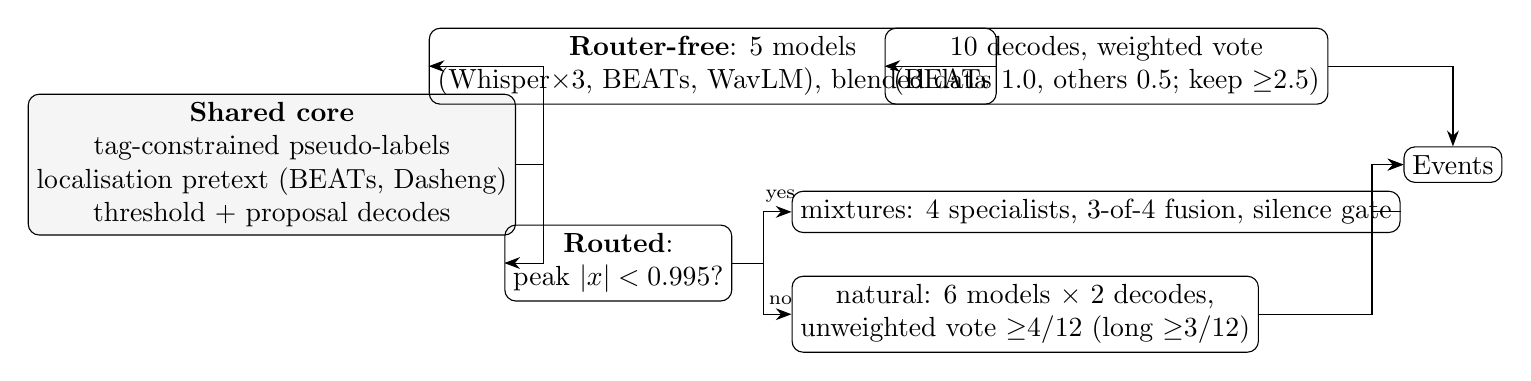
\begin{tikzpicture}[box/.style={draw, rounded corners, align=center, inner sep=3pt}, >={Stealth[length=2mm]}]
\node[box, fill=gray!8] (core) at (0,0) {\textbf{Shared core}\\tag-constrained pseudo-labels\\localisation pretext (BEATs, Dasheng)\\threshold + proposal decodes};
\node[box] (u1) at (5.6,1.25) {\textbf{Router-free}: 5 models\\(Whisper$\times$3, BEATs, WavLM), blended data};
\node[box] (u2) at (10.6,1.25) {10 decodes, weighted vote\\(BEATs 1.0, others 0.5; keep $\geq$2.5)};
\node[box] (r1) at (4.4,-1.25) {\textbf{Routed}:\\peak $|x|<0.995$?};
\node[box, anchor=west] (rs) at (6.6,-0.6) {mixtures: 4 specialists, 3-of-4 fusion, silence gate};
\node[box, anchor=west] (rn) at (6.6,-1.9) {natural: 6 models $\times$ 2 decodes,\\unweighted vote $\geq$4/12 (long $\geq$3/12)};
\node[box] (o) at (15.0,0) {Events};
\draw[->] (core.east) -- ++(0.35,0) |- (u1.west);
\draw[->] (core.east) -- ++(0.35,0) |- (r1.west);
\draw[->] (u1) -- (u2);
\draw[->] (r1.east) -- ++(0.4,0) |- node[pos=0.8, above, font=\scriptsize] {yes} (rs.west);
\draw[->] (r1.east) -- ++(0.4,0) |- node[pos=0.8, above, font=\scriptsize] {no} (rn.west);
\draw[->] (u2.east) -| (o.north);
\draw[->] (rs.east) -| ([xshift=-4mm]o.west) -- (o.west);
\draw[->] (rn.east) -| ([xshift=-4mm]o.west) -- (o.west);
\end{tikzpicture}}
\caption{Overview. Both systems share the core (left). The router-free system (top, our main method) runs one model set and one vote on every clip; the routed system (bottom, our final submission) splits clips by peak level and serves each kind with its own models.}
\label{fig:sys}
\end{figure*}

\begin{figure*}[t]
\centering\footnotesize
\begin{minipage}[t]{0.49\textwidth}
\centering
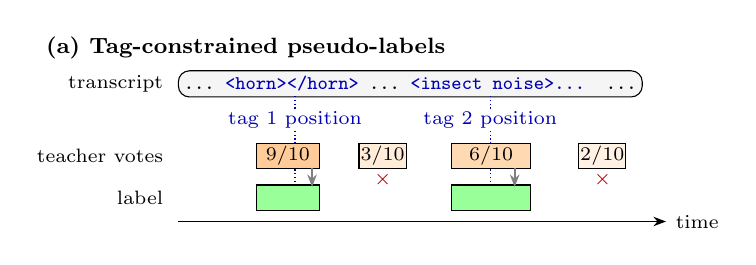
\begin{tikzpicture}[x=6.2mm, y=3.8mm, >={Stealth[length=1.6mm]},
  cand/.style={draw, fill=#1, minimum height=3.2mm, inner sep=0pt, font=\scriptsize},
  lab/.style={anchor=east, font=\scriptsize}]
\node[anchor=west, font=\bfseries\footnotesize] at (-2.9,5.6) {(a) Tag-constrained pseudo-labels};
\node[lab] at (-0.1,4.4) {transcript};
\node[anchor=west, draw, rounded corners, fill=gray!8, inner sep=2pt, font=\ttfamily\scriptsize] at (0,4.4) {\dots\ \textcolor{blue!70!black}{<horn></horn>} \dots\ \textcolor{blue!70!black}{<insect noise>\dots} \dots};
\draw[densely dotted, blue!70!black] (2.4,4.0) -- (2.4,0.3); \draw[densely dotted, blue!70!black] (6.4,4.0) -- (6.4,0.3);
\node[font=\scriptsize, blue!70!black, fill=white, inner sep=1pt] at (2.4,3.2) {tag 1 position};
\node[font=\scriptsize, blue!70!black, fill=white, inner sep=1pt] at (6.4,3.2) {tag 2 position};
\node[lab] at (-0.1,2.0) {teacher votes};
\node[cand=orange!40, minimum width=8mm, anchor=west] at (1.6,2.0) {9/10};
\node[cand=orange!15, minimum width=6mm, anchor=west] at (3.7,2.0) {3/10};
\node[cand=orange!30, minimum width=10mm, anchor=west] at (5.6,2.0) {6/10};
\node[cand=orange!10, minimum width=6mm, anchor=west] at (8.2,2.0) {2/10};
\node[font=\scriptsize, red!70!black] at (4.2,1.2) {$\times$}; \node[font=\scriptsize, red!70!black] at (8.7,1.2) {$\times$};
\node[lab] at (-0.1,0.6) {label};
\node[cand=green!40, minimum width=8mm, anchor=west] at (1.6,0.6) {};
\node[cand=green!40, minimum width=10mm, anchor=west] at (5.6,0.6) {};
\draw[->, thick, gray] (2.75,1.6) -- (2.75,0.95); \draw[->, thick, gray] (6.9,1.6) -- (6.9,0.95);
\draw[->] (0,-0.2) -- (10,-0.2) node[right, font=\scriptsize] {time};
\end{tikzpicture}
\end{minipage}\hfill
\begin{minipage}[t]{0.49\textwidth}
\centering
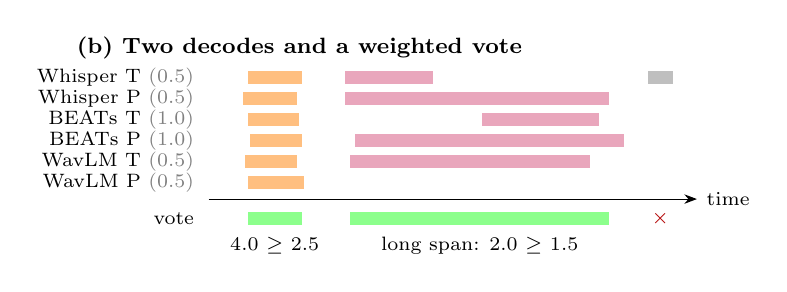
\begin{tikzpicture}[x=6.2mm, y=3.8mm, >={Stealth[length=1.6mm]}, lab/.style={anchor=east, font=\scriptsize}]
\node[anchor=west, font=\bfseries\footnotesize] at (-2.9,5.6) {(b) Two decodes and a weighted vote};
\foreach \y/\n/\w in {4.6/Whisper T/0.5, 3.9/Whisper P/0.5, 3.2/BEATs T/1.0, 2.5/BEATs P/1.0, 1.8/WavLM T/0.5, 1.1/WavLM P/0.5} {
  \node[lab] at (-0.1,\y) {\n\ \textcolor{gray}{(\w)}};
}
\foreach \y/\a/\b in {4.6/0.8/1.9, 3.9/0.7/1.8, 3.2/0.8/1.85, 2.5/0.85/1.9, 1.8/0.75/1.8, 1.1/0.8/1.95} { \fill[orange!50] (\a,\y-0.22) rectangle (\b,\y+0.22); }
\foreach \y/\a/\b in {3.9/2.8/8.2, 2.5/3.0/8.5, 1.8/2.9/7.8} { \fill[purple!35] (\a,\y-0.22) rectangle (\b,\y+0.22); }
\foreach \y/\a/\b in {4.6/2.8/4.6, 3.2/5.6/8.0} { \fill[purple!35] (\a,\y-0.22) rectangle (\b,\y+0.22); }
\fill[gray!50] (9.0,4.38) rectangle (9.5,4.82);
\draw[->] (0,0.55) -- (10,0.55) node[right, font=\scriptsize] {time};
\node[lab] at (-0.1,-0.1) {vote};
\fill[green!45] (0.8,-0.32) rectangle (1.9,0.12); \node[font=\scriptsize, anchor=north] at (1.35,-0.4) {4.0 $\geq$ 2.5};
\fill[green!45] (2.9,-0.32) rectangle (8.2,0.12); \node[font=\scriptsize, anchor=north] at (5.55,-0.4) {long span: 2.0 $\geq$ 1.5};
\node[font=\scriptsize, red!70!black] at (9.25,-0.1) {$\times$};
\end{tikzpicture}
\end{minipage}
\caption{The two core ideas. (a) Tags fix how many teacher candidates become labels; Hungarian matching on time and support picks them (votes out of 10 teacher decodes). (b) T = threshold readout with refiner, P = proposal readout; three of the five models shown. The short event has all six readouts (4.0 $\geq$ 2.5); the long one only Whisper P, BEATs P and WavLM T (2.0), kept by the optional long-span rule (1.5, not in the scored router-free file); the isolated span (0.5) is dropped. Not to scale.}
\label{fig:novel}
\end{figure*}

\section{Introduction and Novelty}
Vaani is a crowd-sourced corpus of Indian speech recorded on phones in homes, streets and fields, so clips are full of non-speech noise (horns, animals, babies, music, breathing); the task is to give the onset and offset of every such event, without naming its category.
It is hard because only 12\% of the 90,635 training clips have verified timestamps, because the test set mixes natural recordings with synthetic mixtures (speech plus pasted noise) that behave very differently, and because on natural recordings even strong models place event edges poorly (event F1 near 0.53, against 0.99 on mixtures).

Our starting observation is that Vaani transcribers already mark noise events in the transcripts with tags such as \texttt{<horn>}\,\dots\,\texttt{</horn>}, which say that an event happened and roughly where, but not exactly when.
We turn this free, weak signal into training labels and build two complete systems around it (Fig.~\ref{fig:sys}).

\textbf{Novelty.}
\begin{itemize}
\item \emph{Tag-constrained pseudo-labels} (Sec.~III-C, Fig.~\ref{fig:novel}a). A teacher ensemble proposes candidate events; the tags' count says how many events the clip has and their positions say which candidates survive, by matching each tag to one candidate on time and support (how many teacher decodes agree). This raises pseudo-label quality by +0.04--0.05 Combined and labels 305k transcribed clips.
\item \emph{Two complementary decodes per model and a duration-aware weighted vote} (Sec.~III-B, Fig.~\ref{fig:novel}b). Every model is read out twice, by a thresholded activity curve whose edges a learned refiner corrects and by an event-proposal head; fusing the two readouts of each model adds 0.012--0.019 over the better single readout, on top of what an ensemble of the same models gains.
\item \emph{A domain-blind, router-free detector} (Sec.~III-E). Five models trained on balanced natural and synthetic data serve every clip with one vote, without detecting the clip's kind, 0.0054 below our routed entry.
\end{itemize}

\section{Task, Data and Rules}
\textbf{Task and metric.}
Clips are 16\,kHz speech, 1.4--21\,s long (median 6.6\,s).
A predicted event matches a reference event when both its onset and offset lie within $\max(0.2\,d, 0.05)$\,s of it ($d$ = reference duration); event F1 counts matches over all events~\cite{mesaros}.
Segment Dice compares predicted and reference activity on 10\,ms frames, averaged over clips.
The score, Combined, is their sum (maximum 2).
Phase 2, the final test round, has 5,517 clips (3,437 natural, 2,080 synthetic) scored on a public leaderboard of each team's best submission.

\textbf{Training data.}
The competition release (\url{ARTPARK-IISc/Vaani-Noise-Event-Dataset}) has three label tiers: 11,111 Gold clips with verified timestamps, 61,640 Silver clips with unverified timestamps, and 17,884 Bronze clips that only say which noise categories occur.
We hold out 2,005 Gold clips of distinct speakers as our validation split.
The organisers also released 1,806 natural and 695 synthetic labelled validation clips, which we use as training data too (four natural models train on the natural ones, all synthetic and router-free models on the synthetic ones).
External data: 321,728 transcribed Vaani clips (\url{ARTPARK-IISc/Vaani-transcription-part}~\cite{vaani}; tags only, no timestamps), 207,268 untranscribed Vaani clips (\url{ARTPARK-IISc/Vaani}), ESC-50 sound events~\cite{esc50}, and the noisy/clean pairs of Track 2 (the datathon's speech-enhancement task), used only to train an enhancement U-Net.
Every competition clip, and every recording behind a validation or test clip, was removed from the transcribed pool; the untranscribed pool, used only without labels, was filtered by clip.
No test labels, test pseudo-labels or manual annotation were used; unlabelled test audio was used twice: its acoustic statistics guided the background of our earliest synthetic mixtures, and its peak levels confirmed the router described in Sec.~III-E.

\section{Method}
\textbf{A. Base model.}
Every model is a convolutional recurrent network (CRNN)~\cite{crnn} on a 10\,ms grid.
Log-mel convolutions are combined with the frames of one pretrained encoder (Table~\ref{tab:pre}), and a bidirectional GRU predicts, per frame, event activity, onset and offset likelihoods, and, through an Event Proposal Network (EPN)~\cite{epn}, the distance to the start and end of the current event.
The loss combines frame and boundary cross-entropy with an IoU loss on the proposals.
Gold labels weigh 1, Silver 0.5--0.9 and pseudo-labels 0.35--0.7 (set per model on validation); Bronze clips get tag-constrained labels from their transcripts (17,373 of 17,884); the rest only supervise a clip-level loss.
Each final model ends a short chain: a model with a frozen encoder, its fine-tuned copy, and a one-epoch \emph{student} trained on labels produced by a \emph{teacher}, an ensemble of earlier models~\cite{noisystudent,cpjku}; a three-model teacher made the earlier labels and a five-model teacher those of the final students.

\textbf{B. Two decodes and the vote.}
A \emph{decode} (or readout) turns a model's frame outputs into events.
The threshold decode thresholds and smooths the activity curve; a small boundary refiner, trained on Gold event edges displaced by up to $\pm$250\,ms, then moves each predicted edge to its most likely true position.
The proposal decode instead reads whole events from the EPN.
The two decodes make different errors, so voting over both helps (Table~\ref{tab:abl}).
A vote fuses the decodes of several models: overlapping spans (IoU $\geq$0.6) form a cluster, each decode adds its model's weight, and a cluster whose summed weight passes a threshold becomes an event with median edges (Fig.~\ref{fig:novel}b). A \emph{long-span rule} lets long clusters, which single decodes often split, pass with less weight; the routed system uses it from 4\,s, while for the router-free system (from 6\,s) it came after our scored submission.

\textbf{C. Tag-constrained pseudo-labels.}
A \emph{teacher} is a set of trained models whose decodes are fused into candidate events, each with a vote count.
For a transcribed clip, we keep the event tags (not \texttt{<noise>}, \texttt{<PAUSE>} or \texttt{[unintelligible]}) and turn each tag into a time prior: a tag occupying the fraction $[a,b]$ of the tag-free text predicts an event centred at $t_{\text{tag}} = \frac{a+b}{2}\,d$ for a clip of duration $d$.
Hungarian matching then assigns each tag exactly one candidate centred at $t_{\text{cand}}$, minimising $3\,|t_{\text{cand}}-t_{\text{tag}}|/d - v/v_{\max}$ (time distance against vote support $v$, with $v_{\max}$ the number of teacher decodes; the factor 3 was chosen on validation); unmatched candidates are discarded, and a tag with no candidate adds no event (Fig.~\ref{fig:novel}a).
On Gold clips, whose transcripts carry the same tags, the tag count equals the verified event count 95.8\% of the time, so the count says how many events to keep and the positions say which.
Scored against our 2,005 held-out Gold clips (which no teacher trained on), the constraint lifts a three-model teacher's labels from 1.1903 to 1.2415 Combined and the five-model teacher's from 1.2145 to 1.2578; for scale, our systems score 1.24--1.25 Combined on natural test clips.
These labels cover 305k transcribed clips and the Bronze clips that have transcripts.

\textbf{D. Pretext task and synthetic mixtures.}
General audio encoders recognise sounds but were not trained to time them, so before fine-tuning BEATs and Dasheng spend 10k steps finding 0--3 ESC-50 sounds pasted into unlabelled Vaani audio; the share of pasted events they localise within the competition's tolerance rises from 0.059 at initialisation to 0.706 (BEATs) and 0.728 (Dasheng).
For the synthetic clips we build mixtures like the organisers': up to six ESC-50, Vaani or organiser noise events (2,213, recovered from their synthetic validation clips by subtracting clean references) pasted into event-free stretches of Gold clips, then peak-normalised.

\textbf{E. Two systems.}
\emph{Router-free (our main method).}
Five students (three Whisper-medium, one BEATs with the pretext, one WavLM) are trained on roughly equal shares of natural clips with tag-constrained labels and synthetic mixtures with exact labels.
One vote fuses their ten decodes on every clip (Whisper and WavLM weigh 0.5, BEATs 1.0; keep at 2.5 of 6).
\emph{Routed (our final submission).}
The organisers' mixtures are peak-normalised to 0.99 while natural clips reach full scale, so a peak test ($|x|<0.995$) separates them exactly; this exploits a property of the release rather than the audio.
Mixtures go to four synthetic specialists (three of four votes, then a gate dropping near-silent spans) and natural clips to six models with an unweighted vote (Fig.~\ref{fig:sys}).


\begin{table}[t]
\caption{Pretrained models: version and source (Hugging Face IDs unless noted) and how many routed (R) and router-free (U) final models use each as encoder.}
\label{tab:pre}
\centering\footnotesize
\begin{tabular}{@{}>{\raggedright}p{2.45cm}>{\raggedright}p{3.35cm}>{\raggedright\arraybackslash}p{2.35cm}@{}}
\toprule
Model & Version / source & Role \tabularnewline
\midrule
Whisper-medium~\cite{whisper} & \url{openai/whisper-medium} & 4 R, 3 U \tabularnewline
WavLM-base-plus~\cite{wavlm} & \url{microsoft/wavlm-base-plus} & 1 R, 1 U \tabularnewline
HuBERT-large~\cite{hubert} & \url{facebook/hubert-large-ll60k} & head init.\ for WavLM \tabularnewline
BEATs iter3+~\cite{beats} & microsoft/unilm & 3 R, 1 U \tabularnewline
Dasheng base~\cite{dasheng} & pip \url{dasheng} 0.0.9 & 2 R \tabularnewline
Enhancement U-Net & ours (Track 2 pairs) & 1 R (extra input) \tabularnewline
\bottomrule
\end{tabular}
\end{table}

\begin{table}[t]
\caption{Phase 2 test set (5,517 clips). Natural / Synthetic give event F1 / Dice on each subset; -- = not logged. $^\dagger$Both derived: overall Dice is the clip-weighted mean of the subset Dice (exact for our routed entry); F1 = Combined $-$ Dice.}
\label{tab:main}
\centering\footnotesize\setlength{\tabcolsep}{2.6pt}
\begin{tabular}{@{}lcccc@{}}
\toprule
System & Combined & F1 / Dice & Natural & Synthetic \\
\midrule
Ours, single model (Sept.) & 1.5883 & -- & .484 / .708 & .996 / .992 \\
\textbf{Ours, routed} & \textbf{1.6168} & .790 / .827 & .526 / .726 & .997 / .992 \\
\textbf{Ours, router-free} & \textbf{1.6114} & .793 / .819$^\dagger$ & .526 / .715 & .993 / .990 \\
\bottomrule
\end{tabular}
\end{table}

\begin{table}[t]
\caption{Evidence per idea. L = label quality vs held-out Gold, V = our validation, O = organisers' natural clips. $^\dagger$Five released router-free models, none trained on V; one saw 2 of the 1,806 O clips. $^\ddagger$95\% speaker-bootstrap interval above zero (\texttt{scripts/ablate\_vote.py}).}
\label{tab:abl}
\centering\footnotesize
\begin{tabular}{@{}>{\raggedright}p{5.0cm}cr@{}}
\toprule
Comparison (A vs B) & On & $\Delta$ Combined \tabularnewline
\midrule
\multicolumn{3}{@{}l}{\emph{Tag-constrained pseudo-labels}} \tabularnewline
Tags vs none, 3-model teacher & L & +0.051 \tabularnewline
Tags vs none, 5-model teacher & L & +0.043 \tabularnewline
Tag count only vs none, 3-model teacher & L & +0.003 \tabularnewline
Student on tag vs plain labels (1 seed) & V & +0.0036 \tabularnewline
\midrule
\multicolumn{3}{@{}l}{\emph{Two readouts and the vote} (columns: V / O)} \tabularnewline
$^\dagger$Vote of 5 models vs 1 model (proposal) & V / O & +0.036 / +0.036 \tabularnewline
$^{\dagger\ddagger}$Both readouts vs proposal-only vote & V / O & +0.019 / +0.012 \tabularnewline
$^\dagger$Both readouts vs threshold-only vote & V / O & +0.028 / +0.028 \tabularnewline
$^{\dagger\ddagger}$Long-span rule vs none & V / O & +0.006 / +0.004 \tabularnewline
\midrule
\multicolumn{3}{@{}l}{\emph{Other components}} \tabularnewline
Pretext task vs none (1 BEATs) & V / O & $-$0.003 / +0.017 \tabularnewline
\bottomrule
\end{tabular}
\end{table}

\section{Results}
\textbf{Test-set scores.}
Our routed system scores 1.6168 (event F1 0.790, Dice 0.827) on the Phase 2 test set (Table~\ref{tab:main}), against 1.5883 for one of our earlier single models; retraining one model with another seed moves the score by up to $\pm$0.002, so smaller differences are not meaningful.
Our router-free submission scores 0.0054 lower with a higher event F1 (0.793, derived): its gap is Dice, the frame overlap, driven by edge placement.

\textbf{What each idea contributes.}
In Table~\ref{tab:abl}, tag positions, not counts, carry the label gain for both teachers, and a student on tag-constrained labels beats one on plain labels from the same audio (+0.0036, one seed).
On held-out clips, voting over five models adds 0.036 and fusing both readouts of each model a further 0.012--0.019 over the better single readout; the pretext task helps on the organisers' clips only.

\textbf{Where natural clips fail.}
For an earlier submission's natural ensemble on the organisers' clips, events under 0.25\,s matched 13\% of the time and 47\% of events over 4\,s were under half covered, while only 127 of 2,531 predictions touched no event: the error is edge placement, not detection.

\textbf{Reproducibility and disclosures.}
The released code reproduces both submissions (one routed clip, empty in our system, carried an earlier submission's prediction); late choices were made on the board, so board gains are optimistic.

\textbf{Conclusion.}
Transcript tags are a free way to constrain pseudo-labels, and voting over two readouts per model gives one detector for both kinds of clip; natural edge placement remains open.

\begin{thebibliography}{12}
\footnotesize
\bibitem{mesaros} A. Mesaros, T. Heittola, and T. Virtanen, ``Metrics for polyphonic sound event detection,'' \emph{Applied Sciences}, 2016.
\bibitem{vaani} ARTPARK, IISc and Google, ``Project Vaani,'' \url{https://vaani.iisc.ac.in}, 2025.
\bibitem{esc50} K. J. Piczak, ``ESC: Dataset for environmental sound classification,'' in \emph{Proc. ACM Multimedia}, 2015.
\bibitem{crnn} E. \c{C}ak{\i}r \emph{et al.}, ``Convolutional recurrent neural networks for polyphonic sound event detection,'' \emph{IEEE/ACM TASLP}, 2017.
\bibitem{epn} F. Schmid, C. I. Tang, S. Parekh, and V. K. Ithapu, ``Sound event detection with boundary-aware optimization and inference,'' arXiv:2601.04178, 2026.
\bibitem{noisystudent} Q. Xie, M.-T. Luong, E. Hovy, and Q. V. Le, ``Self-training with noisy student improves ImageNet classification,'' in \emph{CVPR}, 2020.
\bibitem{cpjku} F. Schmid \emph{et al.}, ``Improving audio spectrogram transformers for sound event detection through multi-stage training,'' arXiv:2408.00791, 2024.
\bibitem{whisper} A. Radford \emph{et al.}, ``Robust speech recognition via large-scale weak supervision,'' in \emph{ICML}, 2023.
\bibitem{wavlm} S. Chen \emph{et al.}, ``WavLM: Large-scale self-supervised pre-training for full stack speech processing,'' \emph{IEEE JSTSP}, 2022.
\bibitem{hubert} W.-N. Hsu \emph{et al.}, ``HuBERT: Self-supervised speech representation learning by masked prediction of hidden units,'' \emph{IEEE/ACM TASLP}, 2021.
\bibitem{beats} S. Chen \emph{et al.}, ``BEATs: Audio pre-training with acoustic tokenizers,'' in \emph{ICML}, 2023.
\bibitem{dasheng} H. Dinkel \emph{et al.}, ``Scaling up masked audio encoder learning for general audio classification,'' in \emph{Interspeech}, 2024.
\end{thebibliography}

\end{document}
